%!TEX root = ../main.tex
\documentclass[float=false, crop=false]{standalone}
\usepackage[subpreambles=true]{standalone}
\begin{document}

\section{Background}
\subsection{Augmented Feedback}
The concept of feedback was popularized when closed-loop control systems were first developed and has since been defined many times~\cite{Wierner1948}.
In the context of this work, a convenient definition of feedback comes from Ramaprasad, ``[f]eedback is information about the gap between the actual level and the reference level of a system parameter which is used to alter the gap in some way~\cite{Ramaprasad1983}.''
The aforementioned ``gap'' is the error and can be conveyed to the operator of a system in a variety of ways.
Feedback can be broadly classified into two types: intrinsic, feedback which is generated from within the context of the action itself, and extrinsic, feedback which is given from an external source~\cite{laurillard1993rethinking}.

Extrinsic feedback, which is also known as augmented feedback, has been extensively studied in the field motor learning~\cite{Sigrist2013}.
In their 2013 review, Sigrist et al. write ``[i]t is generally accepted that augmented feedback, provided by a human expert or a technical display, effectively enhances motor learning~\cite{Sigrist2013}.''
There are a variety of different forms of augmented feedback, that can be further classified by how, when, and by what form the feedback is provided.
For this work, however, we sought to evaluate a type of feedback which was both conceptually simple and could be tied to operational requirements.
With these requirements in mind, we will investigate the effects of concurrent bandwidth feedback.
Concurrent, or real-time, feedback is displayed to the operator while the task is being executed, in contrast to terminal feedback, which is displayed after the task is complete.
Bandwidth feedback is displayed to the operator when some parameter is inside (on-track feedback) or outside (off-track feedback) of an acceptable, predefined tolerance limit.
In our implementation, concurrent bandwidth feedback describes feedback conveyed to the operator when their real-time performance drifts outside of an acceptable tolerance limit.

Experimentation with bandwidth feedback traces its origins to Thorndike's 1927 line-drawing experiment~\cite{thorndike1927law}.
In his experiment, subjects were seated and blindfolded at a table, then asked to draw lines of 3, 4, 5, or 6 inches.
The experiment was divided into two groups of subjects, one group of subjects received no verbal feedback, while the other group was told ``right'' if they were within an 1/8th of an inch of the desired length for the 3 inch line, or 1/4 of an inch for the other three line lengths, and ``wrong'' if they were outside this bandwidth.
Subjects that received the verbal bandwidth feedback improved from an initial median ``right'' percentage of 13\% to 54\% after several training sessions.
The feedback was then removed after these training trials, during which time subjects dropped to a median percentage of 26\%.
This is consistent with the guidance hypothesis (which was not formalized for another fifty years after this experiment was concluded), which states that consistent feedback during the acquisition phase of learning leads to a dependency on the feedback~\cite{salmoni1984knowledge}.
Subjects became dependent on the verbal feedback (extrinsic feedback) rather than their visual or proprioceptive sense (intrinsic feedback) to such an extent that they could no longer perform with the verbal feedback removed.

Payne and Hauty performed one of the first concurrent bandwidth feedback studies in 1955~\cite{payne1955effect}.
In their study, subjects completed a multidimensional pursuit test, which required them to scan four simulated aircraft instruments and counter their drift by adjusting simulated aircraft controls.
Subjects were placed into one of three feedback groups: a control level, where no feedback was provided, a second level, which included a single peripheral visual signal when a deviation in one of the displays occurred, but did not specify which instrument, and a third level, which provided individual indicators for each of the four instruments, and noted the locus of the deviation.
They found a very significant effect between the different feedback groups, with the control group performing the worst, the second level performing better, and the third level performing better still.
Subjects completed the test every hour for a four hour period.
Performance dropped across all three groups as time elapsed, but the performance of the subjects in level three was superior at the end of this period compared to the subjects in the control group at the beginning of the experiment.
They concluded by stating that ``the increment is a positive function of the specificity of the information supplied, it can be ascribed largely to the directive properties of the cues, i.e., the cues impose a more efficient temporal and spatial organization upon [the subject's] scanning behavior~\cite{payne1955effect}.''

Gordon and Gottlieb performed a rotary pursuit study investigating the effects on on-track and off-track concurrent bandwidth feedback in 1967~\cite{Gordon1967}.
Subjects in their study were placed into one of three groups: a control, on-track feedback, and off-track feedback.
The subjects in the bandwidth feedback groups had to track a 0.75 inch by 0.75 inch target with 0.187 inch rigid stylus tip.
For subjects in the on-track feedback group, a light bulb was illuminated when they were on target, and the light bulb was illuminated for subjects in the off-track group when they were not on the target.
While both the on-track and off-track groups performed better than the control group, the off-target group performance was slightly superior.
This finding was consistent with Williams and Briggs for subjects completing their similar task~\cite{williams1962target}.
Additionally, subjects in the feedback groups completed several trials at the end of the experiment without feedback and did not experience the loss of performance which is often seen due to the guidance hypothesis.
This indicates that subjects were able to use the feedback to better learn the task and were not completely dependent on the feedback.
Subjects used their own intrinsic feedback to learn the task, and were able to take advantage of the concurrent bandwidth feedback to both better learn and perform the task without becoming dependent on the external feedback.

In 2011, de Groot et al. investigated the effects of concurrent bandwidth feedback on learning a lane-keeping task in a driving simulator~\cite{DeGroot2011}.
Similar to Gordon and Gottlieb, they investigated the effects of on-track and off-track feedback compared to a control group.
Instead of using a visual indicator, however, de Groot et al. used haptic feedback in the form of a vibrating chair for their feedback groups.
They found that on-target and off-target groups had better lane-keeping performance than the control group, and that, similar to Gordon and Gottlieb and Williams and Brigg, the off-target group performed best.
Retention trials, however, showed that a majority of this performance improvement was lost during when the feedback was removed, which was in accordance with the guidance hypothesis.
The off-target group, though, did still retain some minor performance improvement, which the authors partially attribute to the onset advantage~\cite{fischer2008differential}.
The onset advantage ``suggests that the sudden onset of a stimulus is a more powerful perceptual event than a stimulus offset, facilitating low-level perceptual processing and resulting in faster reaction times~\cite{DeGroot2011}.''
This effect could explain a repeated suggestion that off-track feedback is superior to on-track feedback, even if the effect is, in general, small.
de Groot et al. also measured response time to a secondary task as an estimate of workload, but found no differences across groups.

\subsubsection{SAFER Experiment}
\begin{figure}[tb]
    \begin{center}
        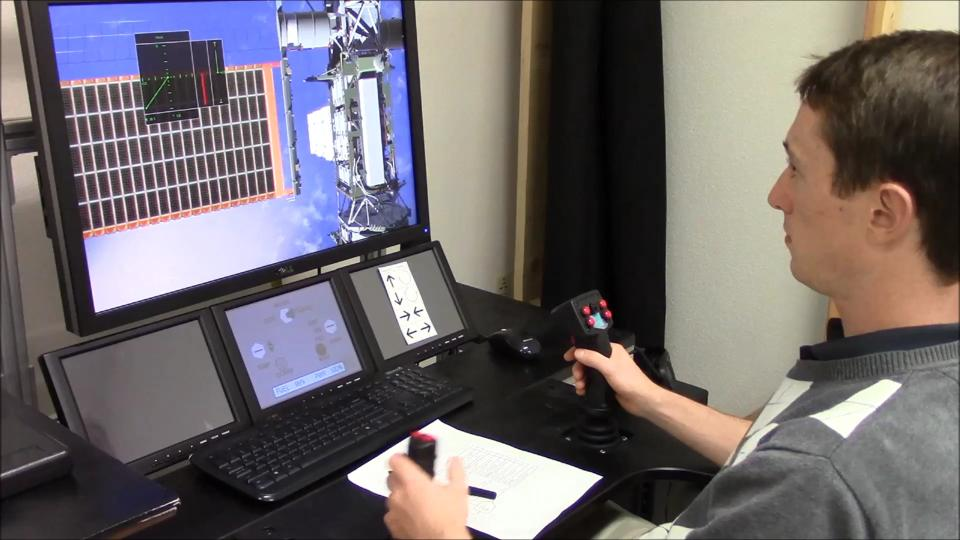
\includegraphics[width=0.8\linewidth]{./../img/SAFER_DangerChris.jpg}
        \caption{A subject from the SAFER experiment seated in the fixed-base simulator~\cite{Karasinski2016Masters}.}
        \label{figure:safersim}
    \end{center}
\end{figure}

Our recent work includes investigations into concurrent bandwidth feedback in a four degree of freedom Simplified Aid for EVA Rescue (SAFER) task~\cite{Karasinski2016Masters, Karasinski2017, Karasinski2016}.
SAFER is a small propulsive jet pack worn during spacewalks for self-rescue~\cite{Vassigh1998}.
Subjects were tasked with flying a SAFER simulation to perform an inspection of the International Space Station's (ISS) solar arrays.
Subjects were initially placed 40 feet away from the solar array and were asked to close to 30 feet and hold this distance for the remainder of the task.
They could gauge their distance from the solar array using the indicator on the guidance display and the out-the-window display.
Subjects were then asked to inspect four ``damaged'' waypoints on the solar array, and were given a guidance display for navigation to the waypoints. %, see Figure~\ref{fig:displays}.
Two vertically arranged displays in the simulator were available to complete the task, see Figure~\ref{figure:safersim}.
The primary display contained an out-the-window view of the solar array and, depending on which group the subject was in, one of the guidance displays. % from Figure~\ref{fig:displays}.
The secondary display located directly below the primary display portrayed information about the subject's current mode, remaining fuel, and a ``comm light''.

\begin{figure}[tb!]
    \begin{center}
        \begin{subfigure}{0.49\textwidth}
            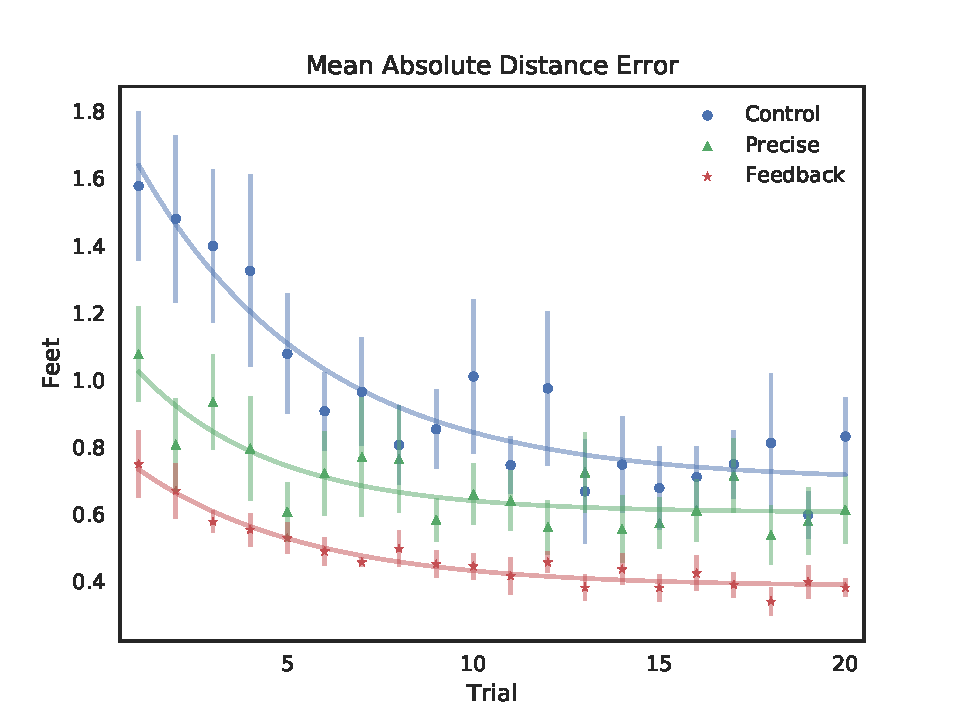
\includegraphics[width=\linewidth]{./../img/Group_absDistErr_clean_fit_30.pdf}
            \caption{Mean absolute distance error, by group.}
            \label{figure:saferdistance}
        \end{subfigure}\hfill
        \begin{subfigure}{0.49\textwidth}
            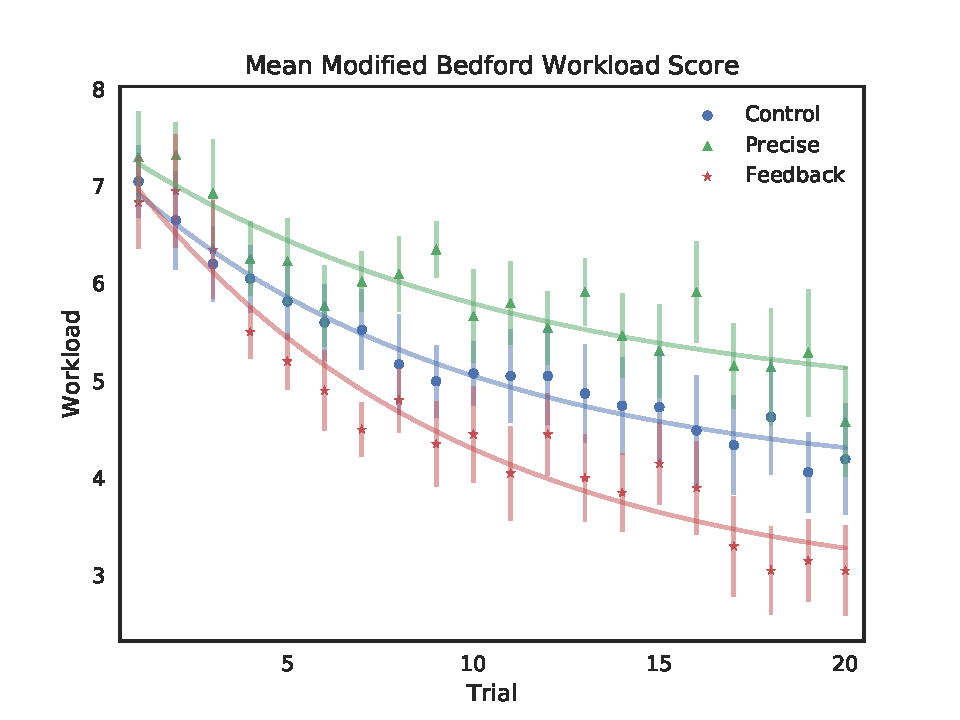
\includegraphics[width=\linewidth]{./../img/Group_Workload_fit_30.pdf}
            \caption{Mean subjective workload rating, by group.}
            \label{figure:saferworkload}
        \end{subfigure}
        \caption{Subjects with CBF performed the best (a) and reported the lowest workload (b). Errors are the standard error of the mean~\cite{Karasinski2016Masters}.}
    \end{center}
\end{figure}

In our experiment, subjects were placed into one of three groups: a control, a high precision augmented feedback group, and a concurrent bandwidth feedback (CBF) group.
Subjects in the high precision group were given an extra significant figure in their guidance display and an analog display which was scaled twice as large (but had half the maximum value) of their flight parameters.
Subjects in the CBF group had two display elements which would change from a green to a red color when the subject's performance was outside a predefined range.
Performance was measured as mean absolute error (MAE) and results across trials are shown in Figure~\ref{figure:saferdistance}.
Both treatment groups performed better than the control group, with the CBF group performing the best and having the least error.
The effects that the treatments had on workload was very different than performance, however.
Subjects in the high precision group reported significantly more workload than the control group, while subjects in the CBF group reported significantly less workload than the control group, see Figure~\ref{figure:saferworkload}.
The concurrent bandwidth feedback also had the added benefit of significantly reducing the amount of time required to train the subjects to their maximum skill level.
Subjects with the CBF performed better on their first trial than subjects in the control group did on their last, which was after approximately two hours on the task.

\subsection{Workload Measurement}
Improving performance, through some kind of feedback or other technique, usually comes at the cost of increased workload, which can lead to a loss of the ability to sustain improved performance.
Workload was defined by Hart and Staveland as ``the perceived relationship between the amount of mental processing capability or resources and the amount required by the task''~\cite{Hart1988}.
More simply put, having a low workload indicates that it would be easy to complete additional tasks, while having a high workload suggests that it would be difficult.

The NASA Task Load Index (NASA-TLX) is one of the most well known and commonly used subjective workload measures.
The NASA-TLX has been in use for thirty years, and has been used and validated over a large variety of tasks~\cite{Hart2006}.
The NASA-TLX is a multidimensional rating scale which uses the magnitude and ranking of six subscales to produce an overall estimate of subjective workload~\cite{Hart1988}.
The six subscales are: Mental Demand, Physical Demand, Temporal Demand, Performance, Effort, and Frustration.
Each of these scales is rated from a 0 (Very Low) to 100 (Very High) scale, with the exception of Performance, which is rated from 0 (Perfect) to 100 (Failure).
After marking a value for each of these subscales, subjects then make fifteen pairwise weightings, allowing them to rate each pair of subscales based on its perceived contribution to their overall workload.
A final, overall workload score is computed by multiplying each subscale's score by the number of times it was chosen in the pairwise weightings, adding these values, and dividing by fifteen.
As certain subscales may be more or less important than others, depending on the task being evaluated, some researchers can drop subscales or simply not compute the overall score.

In addition to subjective measures of workload, there are a variety of techniques which aim to estimate objective workload.
One of the most common objective measurement techniques is the secondary task, which requires subjects to complete the primary task, then use any spare workload to respond to an additional task~\cite{gawron2008human}.
Secondary tasks can provide a measure more sensitive to differences in workload and performance than a single task alone and allow for a common measure between experimental conditions~\cite{slocum1971meaningful}.
Care must be taken, however, to ensure that the secondary task does not intrude upon primary task performance~\cite{williges1979behavioral}.
In our previous studies, we have used a multiple choice reaction time task as an objective workload measurement.
In this secondary task, subjects are presented with several different stimuli, each of which requires a different response~\cite{lysaght1989operator}.
A subject's objective workload can then be inferred by either the percentage of secondary tasks which were correctly responded to within a given time, the number of secondary tasks which were correctly responded to in a trial, or both.
We have previously found this type of task to be accurately tied to subjective workload scales in the aforementioned SAFER task~\cite{Karasinski2017}.

\subsection{Pilot Modeling}
\begin{figure}[tb]
    \begin{center}
        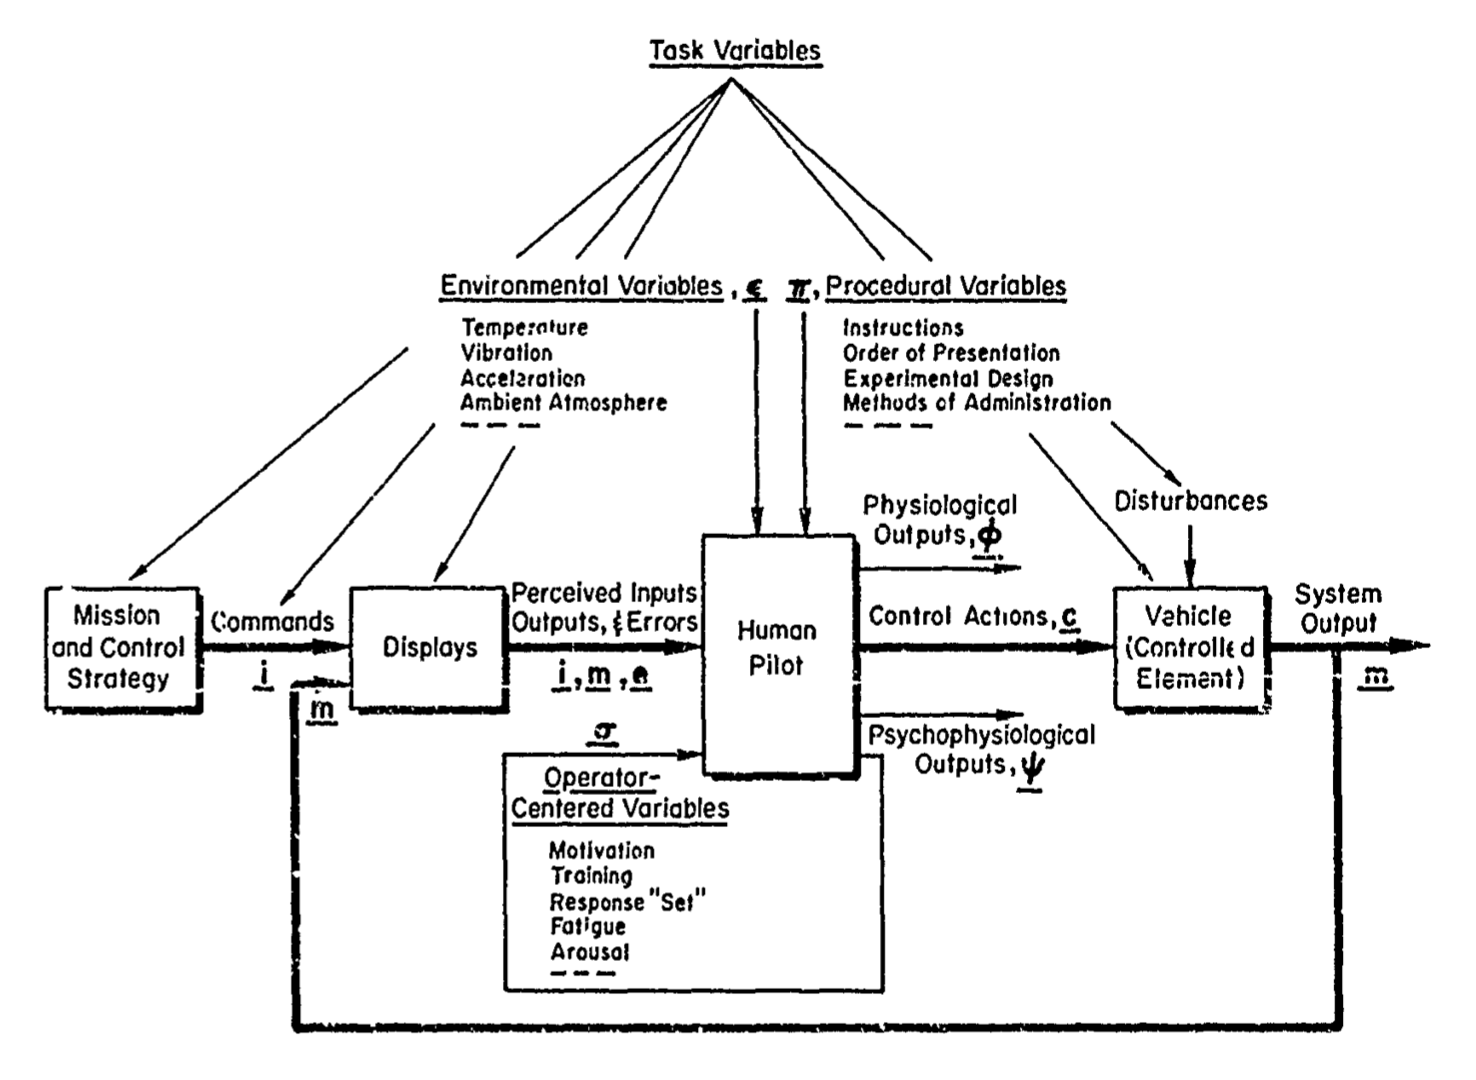
\includegraphics[width=0.8\linewidth]{./../img/Screen Shot 2018-07-25 at 10.37.08 AM.png}
        \caption{Variables affecting the pilot/vehicle system, from~\cite{McRuer1974}.}
        \label{figure:mcruer1974}
    \end{center}
\end{figure}

In addition to popularizing the concept of feedback, the creation of control theory in the early 1940s also provided the tools required for the mathematical modeling of the human pilot.
At the time, new weapons were being created for World War 2 which could only be used effectively with trained operators working in tandem with the machine.
While it was thought that a human could be viewed as a unique kind of servomechanism in the control feedback loop, it was still unclear what factors affected human performance.
Early work by Tustin and others extended the control theory framework and applied these theories to actual human operators~\cite{tustininvestigation}.
Particular interest was focused on ``attempt[ing] to find the laws of relationship of movement and error. In particular, it was hoped that this relationship [would] be approximately linear and so permit well developed theory of `linear servomechanisms' to be applied to manual control in the same way as it applies to automatic following~\cite{tustininvestigation}.''
This would allow for the prediction of human performance and the ability to predict the limits of human control.

These early works were summarized in McRuer's 1957 report, ``Dynamic Response of Human Operators''~\cite{McRuer1957}.
This work evaluated measurements for single-input/single-output (SISO) manual control systems and developed predictive models consistent with this data.
Indeed, McRuer writes, ``[i]t is possible, without doing violence to the data, to obtain describing functions which are generally applicable to the results of the many diverse experiments~\cite{McRuer1957}.''
The report concludes by describing a hypothetical transfer function of the human operator which includes a time delay, a neuromuscular lag, and a gain.
McRuer's early model of the complete pilot/vehicle system is presented in Figure~\ref{figure:mcruer1974}.
McRuer revisited these results in 1974, after three decades of supporting engineering and experimental psychology experiments and was able to further generalize these results to a wide variety of system dynamics~\cite{McRuer1974}.
In his study, McRuer completed a detailed analysis which included the human response to proportional, rate/velocity, and acceleration type controlled element dynamics, see Table~\ref{table:mcruer1974a}.
The result of this report was the now famous ``crossover model,'' which relates the operator and controlled element transfer characteristics by the equation
\begin{align}
Y_c(jw) Y_p(jw) = \dfrac{w_c e^{-jw \tau_e}}{jw}
\end{align}
where $Y_c$ is the controlled element transfer function, $Y_p$ is the approximate human operator transfer function, $w_c$ is the crossover frequency, and $\tau_e$ is the effective time delay of the pilot.
The crossover model is so named as it allows for linear behavior at approximately -20 dB/decade slope in the region of the crossover frequency.
The approximate human operator response to several controlled element transfer functions and their combined open-loop transfer function are presented in Table~\ref{table:mcruer1974b}.
Modeling the human pilot with the crossover enabled a more complete view of the complete pilot/vehicle system, and allowed for human factors recommendations towards the design of new vehicles.
Even today, the crossover model is used as the standard for describing pilot/vehicle systems at the crossover frequency~\cite{McRuer1965, McRuer1974, Xu2017}.

\begin{table}[tb]
    \centering
    \caption{Example Applications of Idealized Controlled Element Forms, adapted from~\cite{McRuer1974}}
    \label{table:mcruer1974a}
    \small
    \begin{tabular}{p{.2\linewidth} *{2}{p{.3\linewidth}}}
        \toprule
            Controlled Element Form & Aerospace Control & Automobile Control \\
        \midrule
            $K_c$ & Attitude control with ACAH system & Speed control \\
            $\dfrac{K_c}{s}$ & Attitude control with a rate command system & Heading control at low to moderate speeds \\
            $\dfrac{K_c}{s^2}$ & Attitude control of a spacecraft with damper off & Longitudinal position control \\
        \bottomrule
    \end{tabular}
\end{table}

\begin{table}[tb]
    \renewcommand{\arraystretch}{2}
    \centering
    \caption{Summary of Human Operator Approximate Characteristics, adapted from~\cite{McRuer1974}}
    \label{table:mcruer1974b}
    \small
    \begin{tabular}{*{3}{c}}
         \toprule
            \thead{Controlled Element\\ Transfer Function\\ $Y_c$} & \thead{Approximate Human Operator\\ Transfer Function\\ $Y_p$} & \thead{Open-Loop\\ Transfer Function\\ $Y_c Y_p$} \\
        \midrule
            $K_c$ & $\dfrac{K_p e^{-\tau_1 s}}{s}$ & $\dfrac{w_c e^{-\tau_e s}}{s}$ \\
            $\dfrac{K_c}{s}$ & $K_p e^{-\tau_2 s}$ & $\dfrac{w_c e^{-\tau_e s}}{s}$ \\
            $\dfrac{K_c}{s^2}$ & $K_p s e^{-\tau_3 s}$ & $\dfrac{w_c e^{-\tau_e s}}{s}$ \\
        \bottomrule
    \end{tabular}
\end{table}

The continued demand for human pilot models for use in informing vehicle design, as well predicting, preventing, and explaining accidents has led to a variety of more complex pilot models since the creation of the crossover model.
A recent review by Xu et al. in 2017 surveyed the state of the art in human pilot modeling and grouped existing models into three classes of models based on: control theory, human physiology, and intelligence techniques~\cite{Xu2017}.
Classical models based on control theory include the McRuer crossover model and optimal control models by Kleinman et al. developed in the early 1970s~\cite{Kleinman1970, Baron1970}.
Of these three overarching sets of models, the models based on human physiology are of the greatest interest here.
Models based on human physiology were developed to understand human pilot perception and control behavior, and include the Hess structural model~\cite{Hess1980, Hess1990, Hess1997}, Hosman's descriptive model~\cite{Hosman1996, Hosman1999}, and the biodynamic model~\cite{Griffin2001}.
Recent intelligence models take advantage of techniques including fuzzy control and neural networks~\cite{Zaychik2006, Gestwa}.

\begin{figure}[tb!]
    \begin{center}
        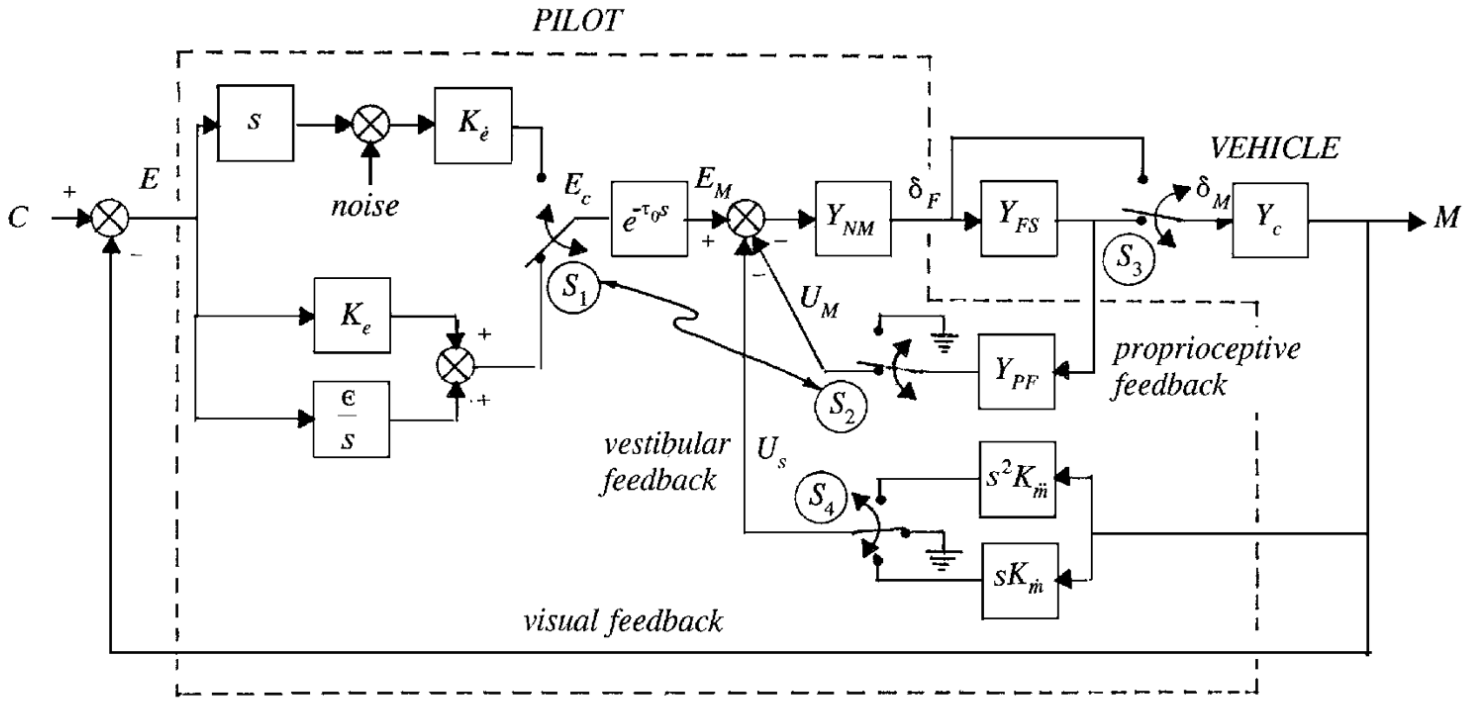
\includegraphics[width=0.8\linewidth]{./../img/Screen Shot 2018-07-31 at 11.21.44 AM.png}
        \caption{The Hess Structural Model of the Human Pilot, from~\cite{Hess1997}.}
        \label{figure:structuralmodel}
    \end{center}
\end{figure}

While the McRuer was very successful in predicting pilot behavior, it it did not attempt ``to describe the underlying structure which contributes to human pilot dynamics~\cite{Hess1980}.''
For this reason, the Hess Structural Model is of particular interest due to the incorporation of multiple sensory channels and models of visual acuity and the time-varying human pilot~\cite{Hess2009}.
The Structural Model includes the effects of the neuromuscular system, the force-feel characteristics of the input device, and the contributions of proprioceptive, vestibular, and visual feedback, see Figure~\ref{figure:structuralmodel}.
One of the key strengths of the Structural Model is the relatively few number of free parameters that need to be set to predict pilot performance.
The model has been used in predicting and evaluating handling qualities and pilot-induced oscillation rating levels for helicopters, Boeing 747, Lockheed C-5A, and twin ducted-fan aircraft~\cite{Hess2013, Andreea-Irina2014, Grant2015}.
Hess has also investigated how pilot control characteristics change with time due to flight anomalies, changing flight dynamics, and sudden increases in task demand~\cite{Hess2009, Hess2016}.
The results of this model have been compared to the results of a human-in-the-loop simulation for a well trained subject, and showed good comparison~\cite{Hess2016}.
Recent work from Bachelder et al. has included modifications to the Structural Model to link pilot performance and workload and to enable the modeling of pulsive pilot behavior~\cite{Bachelder2017, Bachelder2018}.

\end{document}
